\documentclass{article}
\usepackage{amsmath}
\usepackage{graphicx}
\graphicspath{ {code/} }

\title{CVT: Lecture 2}
\date{2018-02-16}
\author{Novitoll}

\begin{document}
    \maketitle
    \pagenumbering{arabic}

    \section{Image Binarization}

    \begin{enumerate}
        \item basic
        \item adaptive
        \item otsu
    \end{enumerate}

    \subsection{Basic}

        \begin{itemize}
            \item thresholding, like everything \textless 127 is black etc.
            \begin{itemize}
                \item cv2.THRESH\_BINARY
                \item cv2.THRESH\_BINARY\_INV
            \end{itemize}
        \end{itemize}

    \includegraphics[scale=0.7]{sudoku-basic-binary-th}

    \subsection{Adaptive}

    More interesting. No hard thresholding like in basic, e.g. usage of mean, Gaussian distrib etc.
    Take some region of the image, like top-left corner 11x11 and use the mean of it. (filtering?)

    \begin{itemize}
        \item adaptive mean thresholding
    \end{itemize}

    \begin{itemize}
        \item adaptive Gaussian thresholding
    \end{itemize}

    Take some region of the image and get Gaussian and get weights per pixel (more pixel is far away of region center - lower weight)

    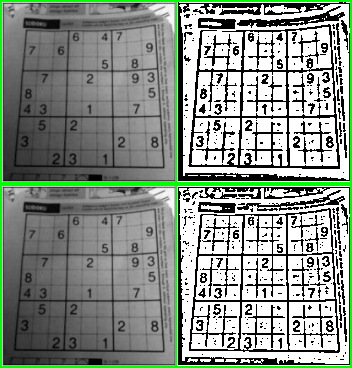
\includegraphics[scale=0.7]{sudoku-adaptive-th}

    \subsection{Otsu}

    Using histogram of pixels count distribution, we can find the boundaries that may binary classify.
    Useful when you have bi-modal distribution.

    \begin{enumerate}
        \item Otsu thresholding
        \item Gaussian blur + Otsu thresholding
    \end{enumerate}

    \includegraphics[scale=0.7]{sudoku-otsu-th}

    \section{Morphology}

    \begin{itemize}
        \item Erosion
    \end{itemize}

    Go near the border of the pixel and remove it
    Iteration = 1

    \includegraphics[scale=0.5]{erosion}

    \begin{itemize}
        \item Dilation
    \end{itemize}

    Go near the border of the pixel and add it
    Iteration = 1

    \includegraphics[scale=0.5]{dilate}

    \begin{itemize}
        \item Opening
    \end{itemize}

    First do the erosion, then do dilation to remove the noise of white
    Iteration = 2

    \includegraphics[scale=0.5]{opening}

    \begin{itemize}
        \item Closing
    \end{itemize}

    First do dilation, then erosion to remove the noise of black
    Iteration = 2

    \includegraphics[scale=0.5]{closing}


\end{document}